\section{Final solution: human following}
\label{sec:follow}

The intention behind developing a UAV control solution that implements tracking and following of humans is to demonstrate the capabilities of the PX4 open-source development platform and its related projects, MAVLink and MAVSDK. The goal is to showcase how complex real-life applications can be designed without relying on expensive proprietary hardware. The follow application requires only a PX4-enabled flight controller installed in an aerial vehicle, a companion computer of appropriate dimensions mounted on board the vehicle, and a camera connected to the companion computer via USB.

In this solution, the vehicle will attempt to detect the relative position of a person in its field of view and follow their movements by changing its yaw and forward velocity to match horizontal movements and distance changes, respectively.
During program execution, the drone can be controlled via an RC controller, an external ground station application or keyboard input directly to the companion computer through, for example, a remote shell (SSH) or a desktop sharing program.

For safety reasons, the follow mechanism only engages when the flight mode on the vehicle is changed to Offboard mode. This can be done through a switch in the RC controller configured in QGroundControl for this purpose. The self-guided control also stops automatically if the connection to the computer is lost or any of the available failsafes are triggered, such as low battery or loss of GPS signal. These safety measures are explained in more detail in Section \ref{subsec:safety}.


When the follow mechanism is engaged, the system continuously retrieves images from the onboard camera. These images are processed using the MediaPipe Pose \cite{mp-pose-paper} computer vision library to extract pose landmarks in the form of 2D coordinates.  Figure \ref{fig:pose-landmarks} shows the features extracted by the external algorithm and their correspondence to the human body. 

\begin{figure}[H]
  \centering
  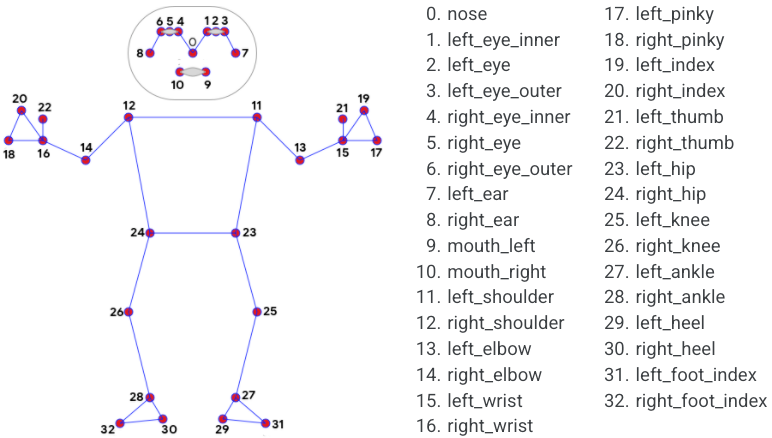
\includegraphics[width=0.8\textwidth, keepaspectratio]{img/pose-landmarks.png}
  \caption{Landmarks extracted from detected human figures by the MediaPipe Pose solution.}
  \source{Adapted from \citetitle{mp-pose} \cite{mp-pose}}
  \label{fig:pose-landmarks}
\end{figure}

The landmarks received from the MediaPipe library are processed inside the application to draw a bounding box around the detected person and validate that they match the expected pose of a person standing up. The bounding box is calculated as a rectangle with its centre in the midpoint between the minimum and maximum x and y coordinates of the landmarks received and a width and height 10\% bigger than the difference between the maximum and minimum coordinates. There are two additional checks to validate that the landmarks extracted from the external library match a person. The first check simply verifies that the height of the bounding box is greater than its width. The second asserts that the features identified with the head, shoulder, hip, knee, and ankle are situated in the correct order from top to bottom of the image. That is, the y coordinate of the head landmark should always be bigger than the y coordinate of the shoulder landmark, which should in turn be bigger than the y coordinate of the hip landmark. These validation checks are implemented in the \texttt{image\_processing}\footnote{\url{https://github.com/l-gonz/tfg-giaa-dronecontrol/blob/main/dronecontrol/follow/image_processing.py}} module.

\begin{figure}[H]
  \centering
  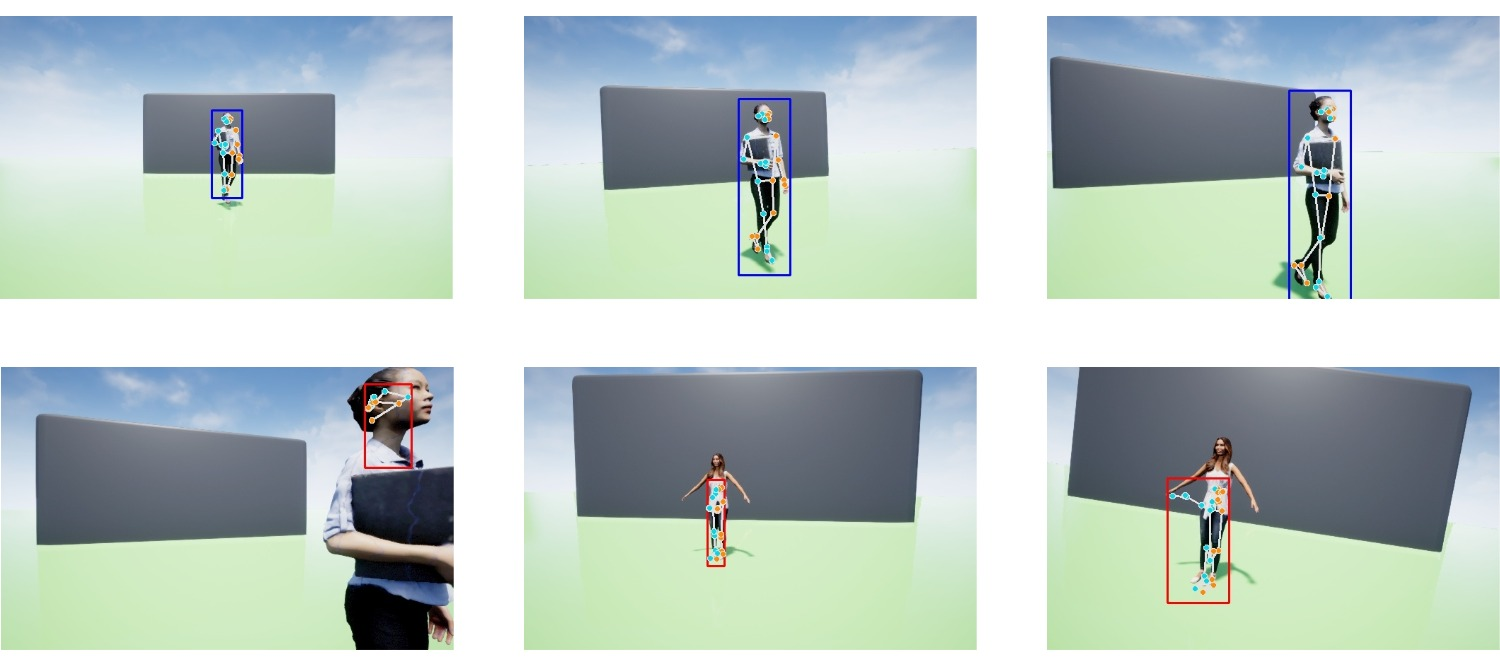
\includegraphics[width=\textwidth, keepaspectratio]{img/pose-validation.jpg}
  \caption{Valid (blue) versus invalid (red) poses detected by the follow solution.}
  \label{fig:pose-validation}
\end{figure}

Figure \ref{fig:pose-validation} shows some examples of the validation checks running on the raw landmarks extracted from an image. Once a valid bounding box is defined around the target person, its position in the image is sent to a control mechanism consisting of two independent PID controllers. These control the vehicle's velocity in the yaw and forward direction, respectively. To ensure controlled movements, the vehicle will stop and hover if it becomes impossible to detect a person in the image or if the detected features do not match the expected pose (invalid bounding box). The vehicle will resume moving when a valid person is detected again.

 
As previously mentioned, DroneVisionControl implements two separate PID controllers to control the vehicle's velocity.
The first one is responsible for controlling the yaw velocity of the vehicle, responding to movement in the horizontal axis of the camera's field of view to attempt to keep the person centred horizontally in the field of view. To achieve this, the process variable or input fed to the controller is x-coordinate of the bounding box position in the camera image, normalized to the width of the image, and the setpoint is the middle of the screen (0.5).
The second PID controller directs the forward velocity of the vehicle to respond to changes in the distance between the followed person and the drone. It adjusts the drone's forward movement to keep the height of the bounding box (as a percentage of the total image height) within a desired range. Since the perceived height in the image depends on the camera perspective, the setpoint for this controller should be determined experimentally for each video source. The setpoint for the physical camera used for flight test is decided as 0.5 by analysing images taken during flight as described in Section \ref{subsec:fl-test-3}. In the AirSim simulator, the same 0.5 setpoint for the forward controller maintains the vehicle and the person separated by approximately 4 meters.

Figure \ref{fig:follow-input-calcs} shows how the inputs for each controller are extracted from the coordinates of the bounding box detected around the figure. Section \ref{subsec:pid-tools} describes the mechanisms the PID controllers employ to translate the input positions to output velocities for the project.
\begin{figure}[H]
  \centering
  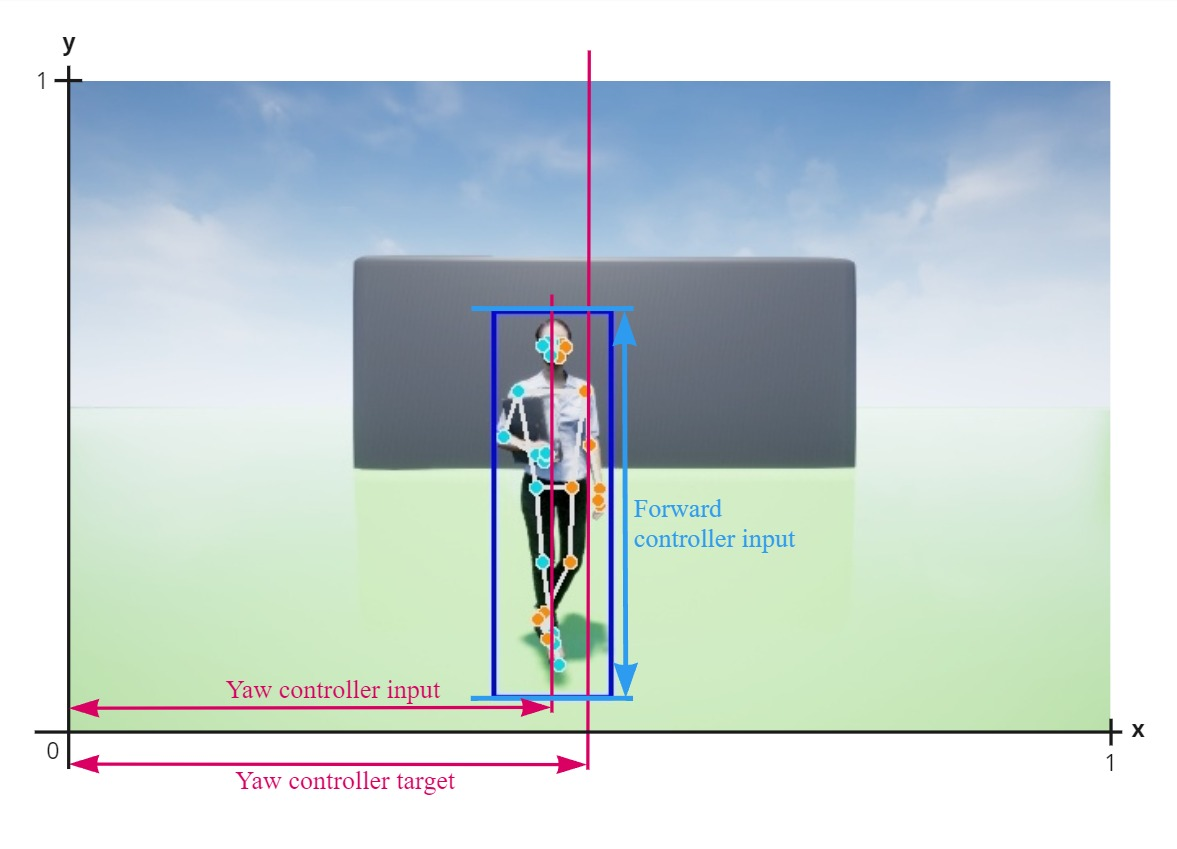
\includegraphics[width=0.8\textwidth, keepaspectratio]{img/pose-calculations.jpg}
  \caption{Calculation of controller inputs from bounding box drawn around the detected figure.}
  \label{fig:follow-input-calcs}
\end{figure}


The structure for follow solution control module\footnote{\url{https://github.com/l-gonz/tfg-giaa-dronecontrol/blob/main/dronecontrol/follow/follow.py}} is summarized in a diagram in Figure \ref{fig:follow-loop}.
In each execution, after connecting to the pilot module with the starting options provided, the main loop runs continuously until the user quits the program.
For each iteration, an image is retrieved, pose features are extracted, and a bounding box is calculated. If the vehicle is in Offboard flight mode, the calculated bounding box is used as input for the PID controllers, which generate velocity outputs to be sent to the pilot module. Keyboard input is also available to send manual control commands to the vehicle according to the mapping in Appendix \ref{app:keyboard}. Unlike in the hand-gesture control solution, all the commands sent here to the pilot module (velocity commands and keyboard input) are run immediately instead of queued for execution. A complete execution of this solution is shown in flight in Section \ref{subsec:fl-test-5}.

\begin{figure}[H]
  \centering
  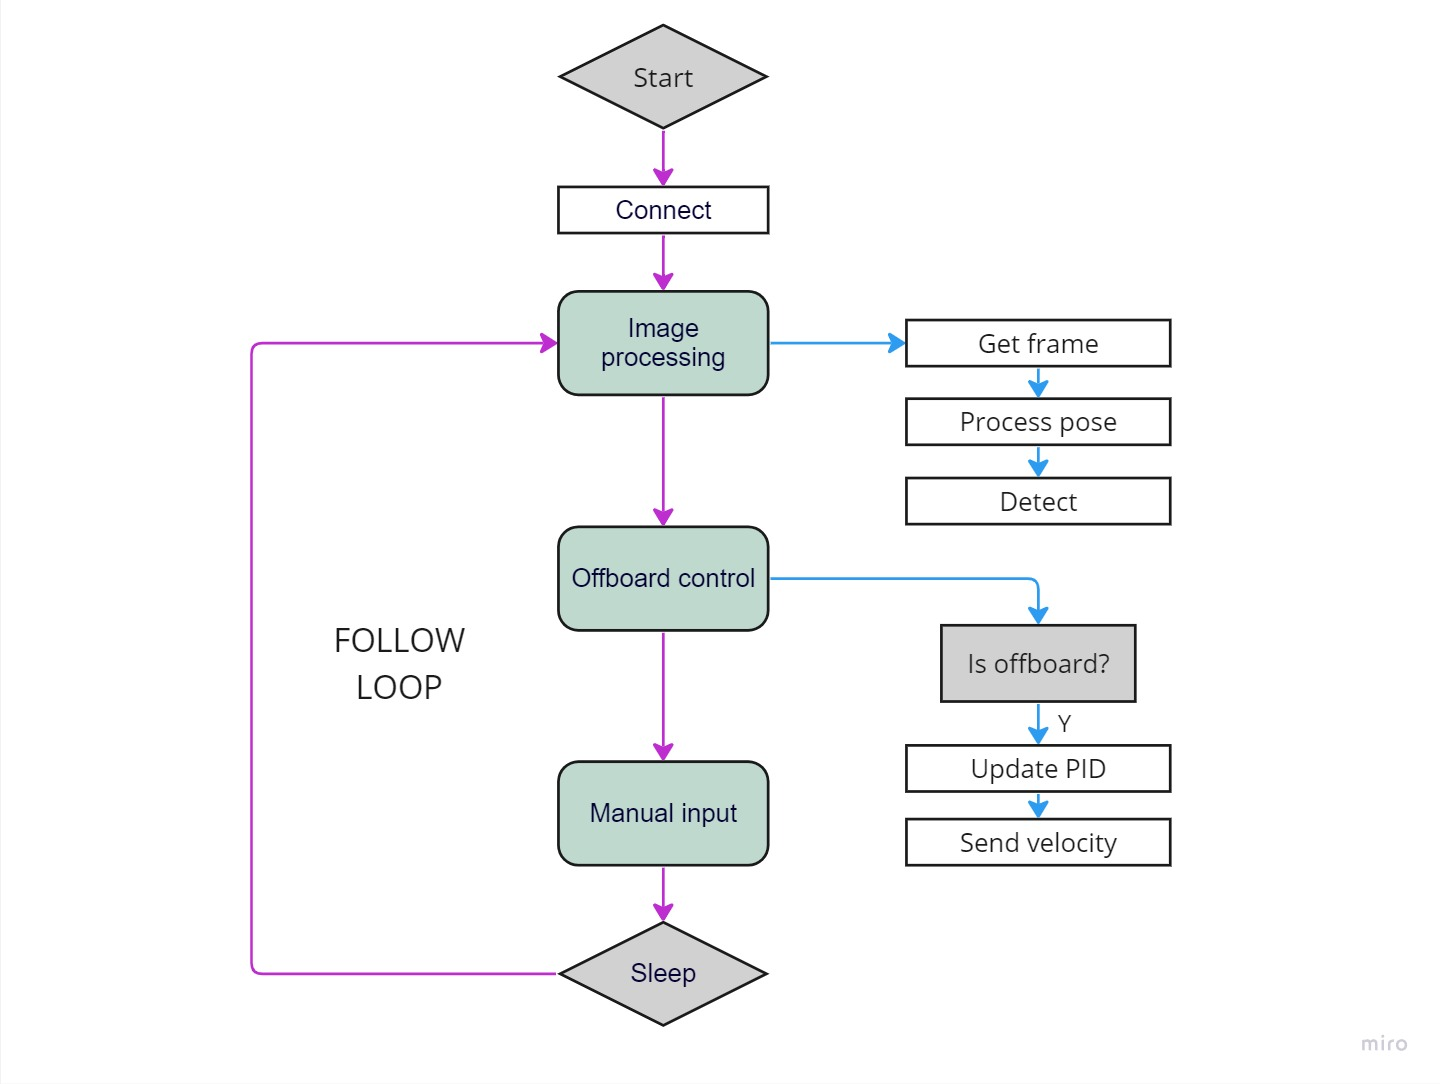
\includegraphics[width=0.9\textwidth, keepaspectratio]{img/follow-loop.jpg}
  \caption{Execution flow for the running loop in the follow control solution.}
  \label{fig:follow-loop}
\end{figure}



\subsection{PID controllers}
\label{subsec:pid-tools}

A \acrfull{pid} is a control loop mechanism commonly used in systems requiring continuously modulated control. One of its biggest advantages is that it relies only on the response of a single measured process variable, not on knowledge or a model of the underlying process. The controller works by continuously calculating an error value from the difference between the received input on a chosen process variable and the desired set point for that variable. From the error value, the output for the controller is calculated according to Equation \ref{eq:pid}. This output is then fed back into the system as a velocity applied to the vehicle. The change in velocity causes a difference in the detected position, which serves as the next input for the controller, creating a closed control loop.

\begin{equation}
    u(t)= K_p e(t) + K_i \int{e(t)dt} + K_d \frac{de(t)}{dt}
    \label{eq:pid}
\end{equation}
\begin{conditions}
u(t)  &   PID control variable \\
K_p   &   proportional gain \\
K_i   &   integral gain \\
K_d   &   derivative gain \\
e(t)  &   error value \\
de    &   change in error value \\
dt    &   change in time
\end{conditions}

The error value is calculated as the difference between the setpoint $r(t)$ and the process variable or input to the controller, $y(t)$:
\begin{equation}
    e(t)= r(t) - y(t)
\end{equation}

The output obtained from the controller is composed of three individual components. The proportional component, characterized by the proportional gain $K_P$, acts proportionally to the current value of the error. On a P-only controller, there is often a remaining control deviation after an equilibrium is reached which causes the set point not to be reached exactly. The integral component, characterized by the integral gain $K_I$, accounts for past error values, accumulating them over time to eliminate the residual error. The derivative component, characterized by the derivative gain $K_D$, attempts to estimate the future trend of the error by reacting to its rate of change, increasing or dampening the control as the error accelerates or decelerates. Each mentioned gain must be particularized to obtain an effective PID controller for the system under study.

While a PID controller is defined by three control terms, certain scenarios adapt better to using only one or two of these terms to achieve precise control. In such instances, the unused parameters are effectively set to zero, resulting in what is commonly referred to as a PI, PD, P, or I controller, depending on the specific control actions involved. PI controllers are often employed when the derivative action might be susceptible to measurement noise. Nonetheless, the integral term remains crucial in many instances, as it is pivotal in guiding the system towards its intended target value. The process of deciding the control parameters, or tuning, for this particular application is described in Section \ref{sec:test-1-pid}.


The velocities that the controllers output are sent to the pilot module to be communicated to the autopilot through MAVLink messages. The autopilot then uses its own internal controllers to translate these velocities into signals for the propeller motors to run at a specific speed and maintain a smooth flight. This intermediate control process creates a discrepancy between the velocities sent from the DroneVisionControl application and those measured by the vehicle's telemetry and will have to be considered when the control parameters are determined. In practice, it will result in the possibility of implementing more aggressive behaviour on the controllers, as the more complex internal autopilot controllers will work to smooth the final trajectory and avoid sudden movements.
%(see Figure \ref{fig:input-measure-diff-todo}).

% \begin{figure}[H]
%   \centering
%   
\includegraphics[width=0.9\textwidth, keepaspectratio]{img/placeholder.png}
%   \caption{}
%   \label{fig:input-measure-diff}
% \end{figure}

The PID controllers in this project are implemented with the help of the open source \texttt{simple-pid} Python library \cite{pid-library}, which supplies all the necessary calculations.
It is only necessary to provide the coefficients or tunings ($K_P$, $K_I$, $K_D$) and the set point (target value) for the controller at the start and then update it periodically with the current input value to receive the output velocity.
In the DroneVisionControl application, it is the internal \texttt{controller} module\footnote{\url{https://github.com/l-gonz/tfg-giaa-dronecontrol/blob/main/dronecontrol/follow/controller.py}} the one that interacts with the external \texttt{simple-pid} library to feed and receive the correct values to the PID controllers calculated from the bounding box around the detected person.

\subsubsection{PID tools}
An additional utility called \texttt{tune\_controller}\footnote{\url{https://github.com/l-gonz/tfg-giaa-dronecontrol/blob/main/dronecontrol/tools/tune_controller.py}} has been developed for tuning and testing the response of the PID controllers. Tuning a PID controller typically involves testing different combinations of coefficients empirically. The \texttt{tune\_controller} tool facilitates this process by allowing users to specify a range of potential coefficients and testing the system's step response using images retrieved from AirSim and a simulated flight controller (SITL or HITL). The tool sets up a simulated person in an offset position from the target centre, engages the controller with the test values, and plots the detected position input and calculated velocity output on a graph for analysis. After each test, the vehicle returns to the starting position to reset the environment for the next coefficient to be checked. The tool can be executed using the command \texttt{dronevisioncontrol tools tune} and can be started with the option \texttt{--yaw} or \texttt{--forward} to tune a specific controller while deactivating the other one. Each coefficient can be tested individually by providing fixed values for the other two parameters.


\subsection{Safety measures}
\label{subsec:safety}

The DroneVisionControl application implements a very experimental vision-based guidance system.
Therefore, to carry out flight tests in real-life conditions, it is necessary to ensure that there are sufficient safety mechanisms to prevent accidents. The software-based safety features used in this project can be divided into those offered by the external PX4 autopilot and those developed as part of the DroneVisionControl application.

The PX4 autopilot offers various safety configuration options, known as failsafes, documented in \citetitle{px4-docs-safety} \cite{px4-docs-safety}. These failsafes detect undesired conditions during flight and include detecting a lost connection to the companion computer while in Offboard mode, a loss of RC transmitter link or GPS position, low battery levels during flight, and unexpected flipping of the vehicle. When any of these conditions are detected, the autopilot triggers a flight mode change to either Hold (hover) or Return (fly back to takeoff position and land), ensuring the safety of the drone and its surroundings. The failsafes' failure conditions and actions triggered in response can be configured through QGroundControl, the PX4 console or an offboard API (MAVSDK).

Additionally, operator control can play a vital role in ensuring safety during flight by leveraging QGroundControl to map PX4 commands to switches in an RC controller. This allows the operator to use an RC controller with a configured switch to deactivate Offboard mode at any time during a flight controlled by the follow solution. This action causes the vehicle to disregard instructions from the companion computer and assume control through GPS-assisted or manual flight modes. A secondary switch can also be configured as a kill switch, allowing for an immediate stop of all motor outputs when needed. This feature is particularly useful in situations where the vehicle is on the ground and has trouble taking off to reduce the risk of propeller damage if the vehicle flips.

On the DroneVisionControl side, the computer vision module that interacts with the external pose detection library incorporates several checks to validate that the received results match specific features associated with a standing human figure. Any detections that do not pass these tests are rejected as invalid as described in \ref{sec:follow}. If the detection output is invalid or empty (nothing detected in the image) is received, the vehicle immediately enters Hold flight mode. In this mode, any velocity commands are discarded, and the drone hovers in its current position. When a valid person is detected again, the follow mechanism resumes controlling the vehicle's velocity. In addition to detection validation, the application incorporates output limits for the PID controllers and the pilot module, which limit the maximum possible velocity of the vehicle at all times during the execution.


By integrating the safety features of PX4 with those developed for this project, the DroneVisionControl application aims to mitigate potential risks and ensure safe flight operations under real-life conditions.
